\chapter{System Design and Pipeline Architecture}
\label{ch:design}

% Four monospace paths in four lines leave TeX no room to break, and the
% longest ran 30 pt past the margin. sloppypar lets it stretch the interword
% spaces instead of overflowing; \allowbreak supplies the break points a
% \texttt{} token does not otherwise have.
\begin{sloppypar}
The analysis pipeline consists of twelve numbered scripts in
\texttt{sepsis/\allowbreak project/}, executed in sequence after the
pre-registration document \texttt{00\_\allowbreak preregistration.md}. Each
stage reads defined upstream outputs and writes stage-specific results to
\texttt{sepsis/\allowbreak project/\allowbreak output/}, leaving the source data
unchanged. This chapter describes the architecture, stage interfaces,
validation checks and reproducibility controls; the statistical rationale for
each step is given in Chapter~\ref{ch:methodology}. Figure~\ref{fig:pipeline_dag}
shows the data flow, and Appendix~\ref{app:stages} lists each stage's inputs and
outputs.
\end{sloppypar}


\section{Design Principles}
\label{sec:design_principles}

\paragraph{Read-only, streamed source data.}
Large source tables (\texttt{chartevents}, 3.5\,GB compressed;
\texttt{labevents}, 2.6\,GB) are queried through DuckDB with the cohort and
item-identifier filters pushed into the scan, so the full tables are never
loaded into memory. Source directories are read-only, and all derived data are
written to \texttt{output/}, so a run never alters the inputs of the next.

\paragraph{Centralised configuration.}
\texttt{config.R} defines every path, identifier, window, threshold, seed,
family size, event floor and feature list used by more than one stage. Because
the study varies label definitions, a constant duplicated across scripts could
diverge without warning and be indistinguishable from a finding. The
model-fitting and transport stages read the same declared feature vector and
verify names and order before scoring.

\paragraph{Fail-fast interface validation.}
Interface violations terminate the pipeline with an error rather than letting
it continue on inferred or incomplete inputs. Selecting predictors by
intersecting a declared list with the columns present would silently omit any
predictor whose name did not match while the model still fitted, so
\texttt{require\_features()} stops a stage when a declared predictor is absent.
Runtime assertions also check key invariants, including the bounds of the
Utility Score (a threshold above every prediction must score zero, and no
operating point may exceed one) and that the label variants produce distinct
external onset sets.

\paragraph{Independent stages and isolated outputs.}
Each stage corresponds to a distinct analytical operation and writes reusable
intermediate outputs in Parquet, so individual stages can be rerun and
validated independently. Stage 12 operates only on stored predictions, so
intervals and multiplicity corrections can be recomputed without refitting any
model. Variant-specific and ablation analyses are written to separate outputs,
so additional analyses can be run without overwriting pre-registered fits.

\begin{figure}[H]
    \centering
    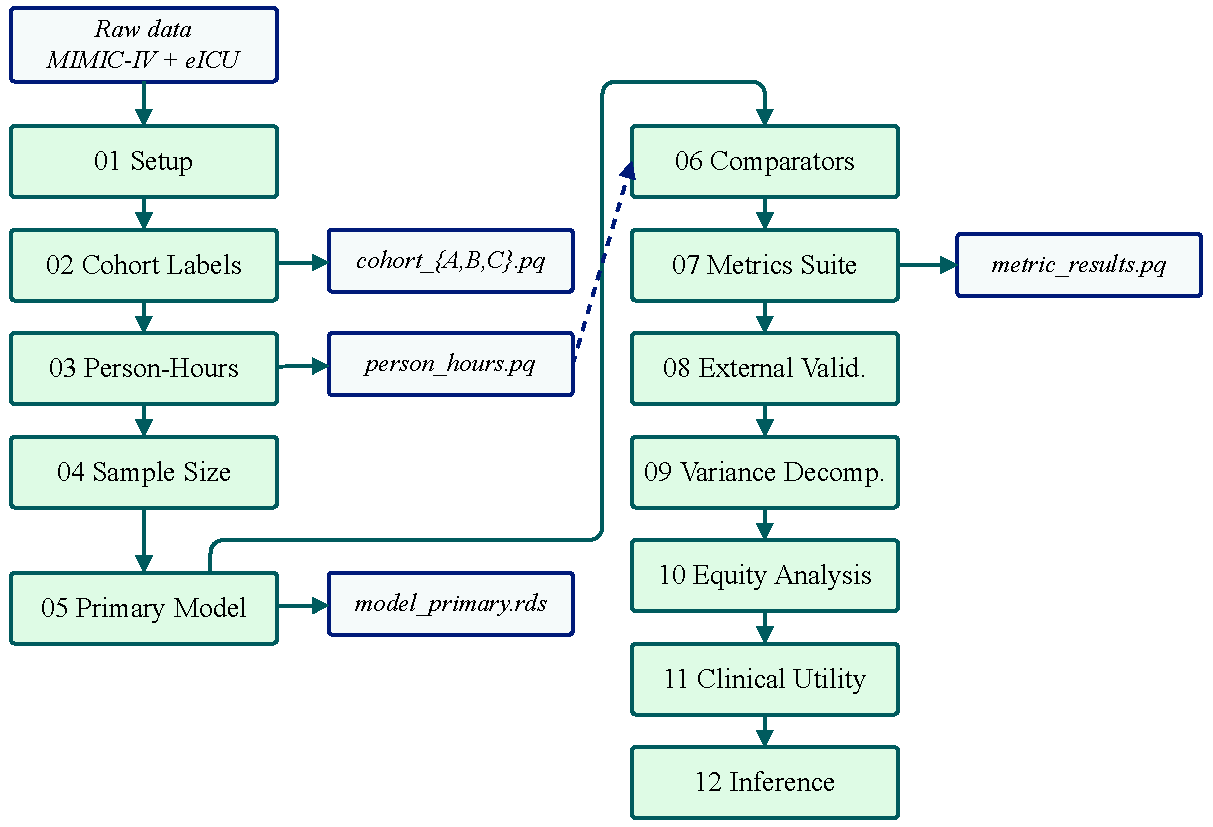
\includegraphics[width=0.95\textwidth]{figures-img/fig4.1_pipeline_dag.pdf}
    \caption{Pipeline data flow. Each box is a single script; italic nodes are
    output files. Raw MIMIC-IV and eICU-CRD data are read-only.}
    \label{fig:pipeline_dag}
\end{figure}


\section{Configuration and Utilities}

\texttt{config.R} defines the shared pipeline parameters, including data paths,
cohort criteria, antibiotic name lists, MIMIC-IV item identifiers, label
variant definitions, split boundaries, prediction framing constants, equity
variable names and Utility Score parameters.

\texttt{utils.R} provides common input/output, data-processing, validation and
diagnostic functions: a DuckDB-backed streaming reader, Parquet wrappers,
datetime parsing, last-observation-carried-forward (LOCF) imputation, feature
checks and Schoenfeld test wrappers. It also supplies the score function that
the \texttt{sandwich} package lacks for \texttt{multinom} fits: for row $i$ and
non-reference category $k$, the score for the coefficient on covariate $j$ is
$x_{ij}(y_{ik} - p_{ik})$, which together with the retained Hessian yields the
stay-clustered covariance of Section~\ref{sec:primary_model_spec}.


\section{Data Preparation (Stages 01--04)}

\subsection{Stage 01: Setup Validation}

\texttt{01\_setup.Rmd} verifies that the required MIMIC-IV source tables are
present and terminates if any is unavailable.

\subsection{Stage 02: Cohort Extraction and Labelling}

\texttt{02\_cohort\_labels.Rmd} constructs the base cohort, attaches the equity
variables, and generates cohort-level labels for Variants A--C and the
post-hoc alternative labels described in Sections~\ref{sec:label_variants}
and~\ref{sec:alt_labels}. Variant D's onsets and Variant F's re-timed onsets
need the hourly SOFA trajectory and are derived in Stage 03. The post-hoc
variants are excluded from the pre-registered variant set in \texttt{config.R}
and written to separate files, so they cannot enter H1 or the decomposition
table.

\subsection{Stage 03: Person-Hour Table Construction}

\texttt{03\_person\_hours.Rmd} expands each stay into hourly rows and is the
only analytical stage that queries the full-size event tables directly. For
each person-hour:

\begin{itemize}
    \item Vitals and labs are LOCF-imputed from the most recent measurement.
    \item Six-hour rolling slopes are computed for heart rate, respiratory
    rate and MAP.
    \item Vasopressor indicators are set from concurrent infusions.
    \item Missingness flags are set for each lab test.
    \item The competing-event code (0/1/2/3) is assigned based on the hour's
    relationship to onset, discharge, or death.
    \item The temporal split group is assigned from the stay's admission year.
    \item Treatment anchor timestamps (first antibiotic, first culture) are
    recorded.
\end{itemize}

\subsection{Stage 04: Sample Size Calculation}

\texttt{04\_sample\_size.Rmd} implements the stay-level sample-size assessment
of Section~\ref{sec:sample_size} and also produces a person-hour reference
calculation, labelled as such because person-hours are not independent.


\section{Modelling (Stages 05--06)}

\subsection{Stage 05: Primary Model}

\texttt{05\_primary\_model.Rmd} fits the primary model of
Section~\ref{sec:primary_model_spec} for each requested label variant under the
temporal and random splits. It validates the declared feature set, applies the
fixed ridge penalty, and logs the convergence flag alongside the largest fitted
coefficient, flagging any fit in which $\max|\beta|$ exceeds 20. It writes the
fitted models, coefficients, coefficient covariances and test predictions;
the full and ablated specifications (Section~\ref{sec:ablation_method}) are
written to separate outputs.

\subsection{Stage 06: Comparator Models}

\texttt{06\_comparators.Rmd} fits the GBT and the Cox comparator of
Sections~\ref{sec:gbt_spec} and~\ref{sec:cox_spec}, runs the Schoenfeld tests,
and computes NEWS2, qSOFA and SIRS at each person-hour. The GBT is fitted under
both splits and on the ablated feature set with identical hyperparameters, and
its early-stopping holdout is drawn from training stays only; GBT feature
importance is exported for each variant. The rule-based scores never use the
ablated features, and the Cox comparator is not ablated.


\section{Evaluation (Stages 07--11)}

\subsection{Stage 07: Metrics Suite}

\texttt{07\_metrics\_suite.Rmd} evaluates stored predictions using the metrics
of Section~\ref{sec:metrics} and writes split-specific, label-specific and
ablation result tables. The utility threshold grid is evaluated in a single
sorted pass, and the Utility Score invariants are asserted automatically. A
stand-alone Python implementation of the same scoring rule,
\texttt{utility\_score.py}, is kept in step with the stage so that the two
implementations can be cross-checked.

\subsection{Stage 08: External Validation on eICU-CRD}

\texttt{08\_external\_validation.Rmd} applies the frozen MIMIC-IV models to
harmonised eICU-CRD features without retraining. It produces three separate
analyses: the Sepsis-3 variants on the microbiology-covered sub-cohort, the
antibiotic-only sensitivity analysis on the full cohort, and the post-hoc
Variant D analysis on the full cohort (Section~\ref{sec:label_transport}).
\texttt{check\_model\_features()} rebuilds each design matrix from the declared
feature vector and verifies compatibility before scoring. Runtime guards
require the three Sepsis-3 variants to produce distinct onset sets, and keep
the post-hoc Variant D output and the pre-registered external output in
separate files, so a post-hoc label cannot enter H5.

\subsection{Stage 09: Variance Decomposition}

\texttt{09\_variance\_decomposition.Rmd} assembles the one-factor-at-a-time
AUROC contrasts defined in the pre-registration and generates the label-anchor
attribution and onset-agreement summaries. It records the pre-registered H5
contrast as undefined and stores the substituted AUROC transport contrast
separately (Section~\ref{sec:h5}).

\subsection{Stage 10: Equity Analysis}

\texttt{10\_equity\_analysis.Rmd} estimates subgroup discrimination and label
sensitivity for the equity variables available in MIMIC-IV: race, language and
insurance. It applies the estimation and interpretation floors defined in
Section~\ref{sec:inference}.

\subsection{Stage 11: Clinical Utility Metrics}

\texttt{11\_clinical\_metrics.Rmd} generates the calibration, decision-curve,
fixed-sensitivity, per-patient alert, alarm-episode and lead-time outputs
defined in Section~\ref{sec:metrics}, for both MIMIC-IV and eICU-CRD.


\section{Inference and Multiplicity (Stage 12)}

\texttt{12\_inference.Rmd} reads stored predictions and produces stay-level
bootstrap intervals, the multiplicity-adjusted confirmatory results, the
exploratory-family corrections and the analysis register
(Section~\ref{sec:inference}). It resamples ICU stays rather than
person-hours. Reduced-replicate settings for smoke tests are documented in
Appendix~\ref{app:repro}; reported results always use the replicate counts
fixed in \texttt{config.R}.


\section{Reproducibility}

The pipeline is orchestrated by \texttt{run\_\allowbreak pipeline.R} (or the
equivalent \texttt{run\_\allowbreak pipeline.sh}), which executes all stages
sequentially or by phase, renders each stage to PDF in \texttt{output/pdf/},
and writes per-stage and combined run logs to \texttt{output/logs/}.
Intermediate outputs are Parquet, and small result tables are also written as
CSV. The end-to-end run that produced the reported results took about two and
a half hours on an Apple silicon workstation, dominated by Stage 05.
\texttt{thesis\_constants.R} generates the numerical values used in this thesis
from the pipeline result tables (Appendix~\ref{app:repro}).

\subsection{Fixed Random Seed}

The fixed seed 42 is defined centrally and applied to stochastic splitting,
the sample-size procedure, model fitting and bootstrap resampling, to support
repeatability within the analysis environment. The temporal partition is
deterministic, because it is defined by admission year. Seeding does not by
itself guarantee bitwise reproducibility across environments: GBT results were
monitored when comparing runs, because they are the component most likely to
vary slightly across library builds or architectures (Appendix~\ref{app:repro}).
The pipeline can be rerun on a credentialed MIMIC-IV v3.1 installation by
setting \texttt{MIMIC\_RESEARCH\_ROOT} to the directory containing the
\texttt{data/} folder.

\subsection{Code Availability}
\label{sec:code_availability}

The pipeline is held in a public version-controlled repository at
\url{\repourl}, released under the \repolicence. The repository contains the source code but no MIMIC-IV or eICU-CRD records,
derived person-hour tables or fitted model objects, because the PhysioNet data
use agreement (Section~\ref{sec:ethics}) prohibits redistribution of the
underlying data. Reproduction therefore requires independent PhysioNet
credentialing for both databases. Appendix~\ref{app:code} describes the
repository layout, the reproduction procedure and the scope of the licence.
